\documentclass[11pt]{article}
\usepackage[a4paper,margin=18mm,headheight=14pt,footskip=10mm]{geometry}
\usepackage[T1]{fontenc}
\usepackage{lmodern,microtype,amsmath,amssymb,adjustbox,xcolor,graphicx}
\usepackage{quantikz}
\usepackage{fancyhdr,hyperref,caption,needspace}
\hypersetup{colorlinks=true,linkcolor=blue,urlcolor=blue,
pdftitle={C4-Helix magic preparation: circuit, state, and fault tolerance}}
\definecolor{ink}{HTML}{203044}
\definecolor{cat}{HTML}{986F14}
\definecolor{gauge}{HTML}{148E9E}
\definecolor{groupa}{HTML}{367AAF}
\definecolor{groupb}{HTML}{D47D28}
\definecolor{groupc}{HTML}{378957}
\definecolor{groupd}{HTML}{8863AF}
\definecolor{groupe}{HTML}{CA5D85}
\setlength{\parindent}{0pt}
\setlength{\parskip}{5pt}
\setlength{\emergencystretch}{2em}
\clubpenalty=10000
\widowpenalty=10000
\displaywidowpenalty=10000
\captionsetup{font=small,labelfont=bf,hypcap=false}
\pagestyle{fancy}\fancyhf{}
\fancyhead[L]{\small\color{ink}C4-Helix / procedure and proof}
\fancyhead[R]{\small Single gauging cycle}
\fancyfoot[R]{\thepage}
\renewcommand{\headrulewidth}{.3pt}
\begin{document}
{\LARGE\bfseries\color{ink}C4-Helix magic preparation\par}
\vspace{2mm}{\large\bfseries\color{ink}circuit, state, and fault tolerance\par}
\vspace{3mm}
This note follows one complete preparation attempt in execution order. At each stage it gives the ideal state, the physical circuit, and a fault example explaining the required protection. The protocol uses one gauging/ungauging cycle, three rounds of checks while gauged, and postselection: a failed required test rejects the entire attempt.

\begin{center}\begin{minipage}{\linewidth}
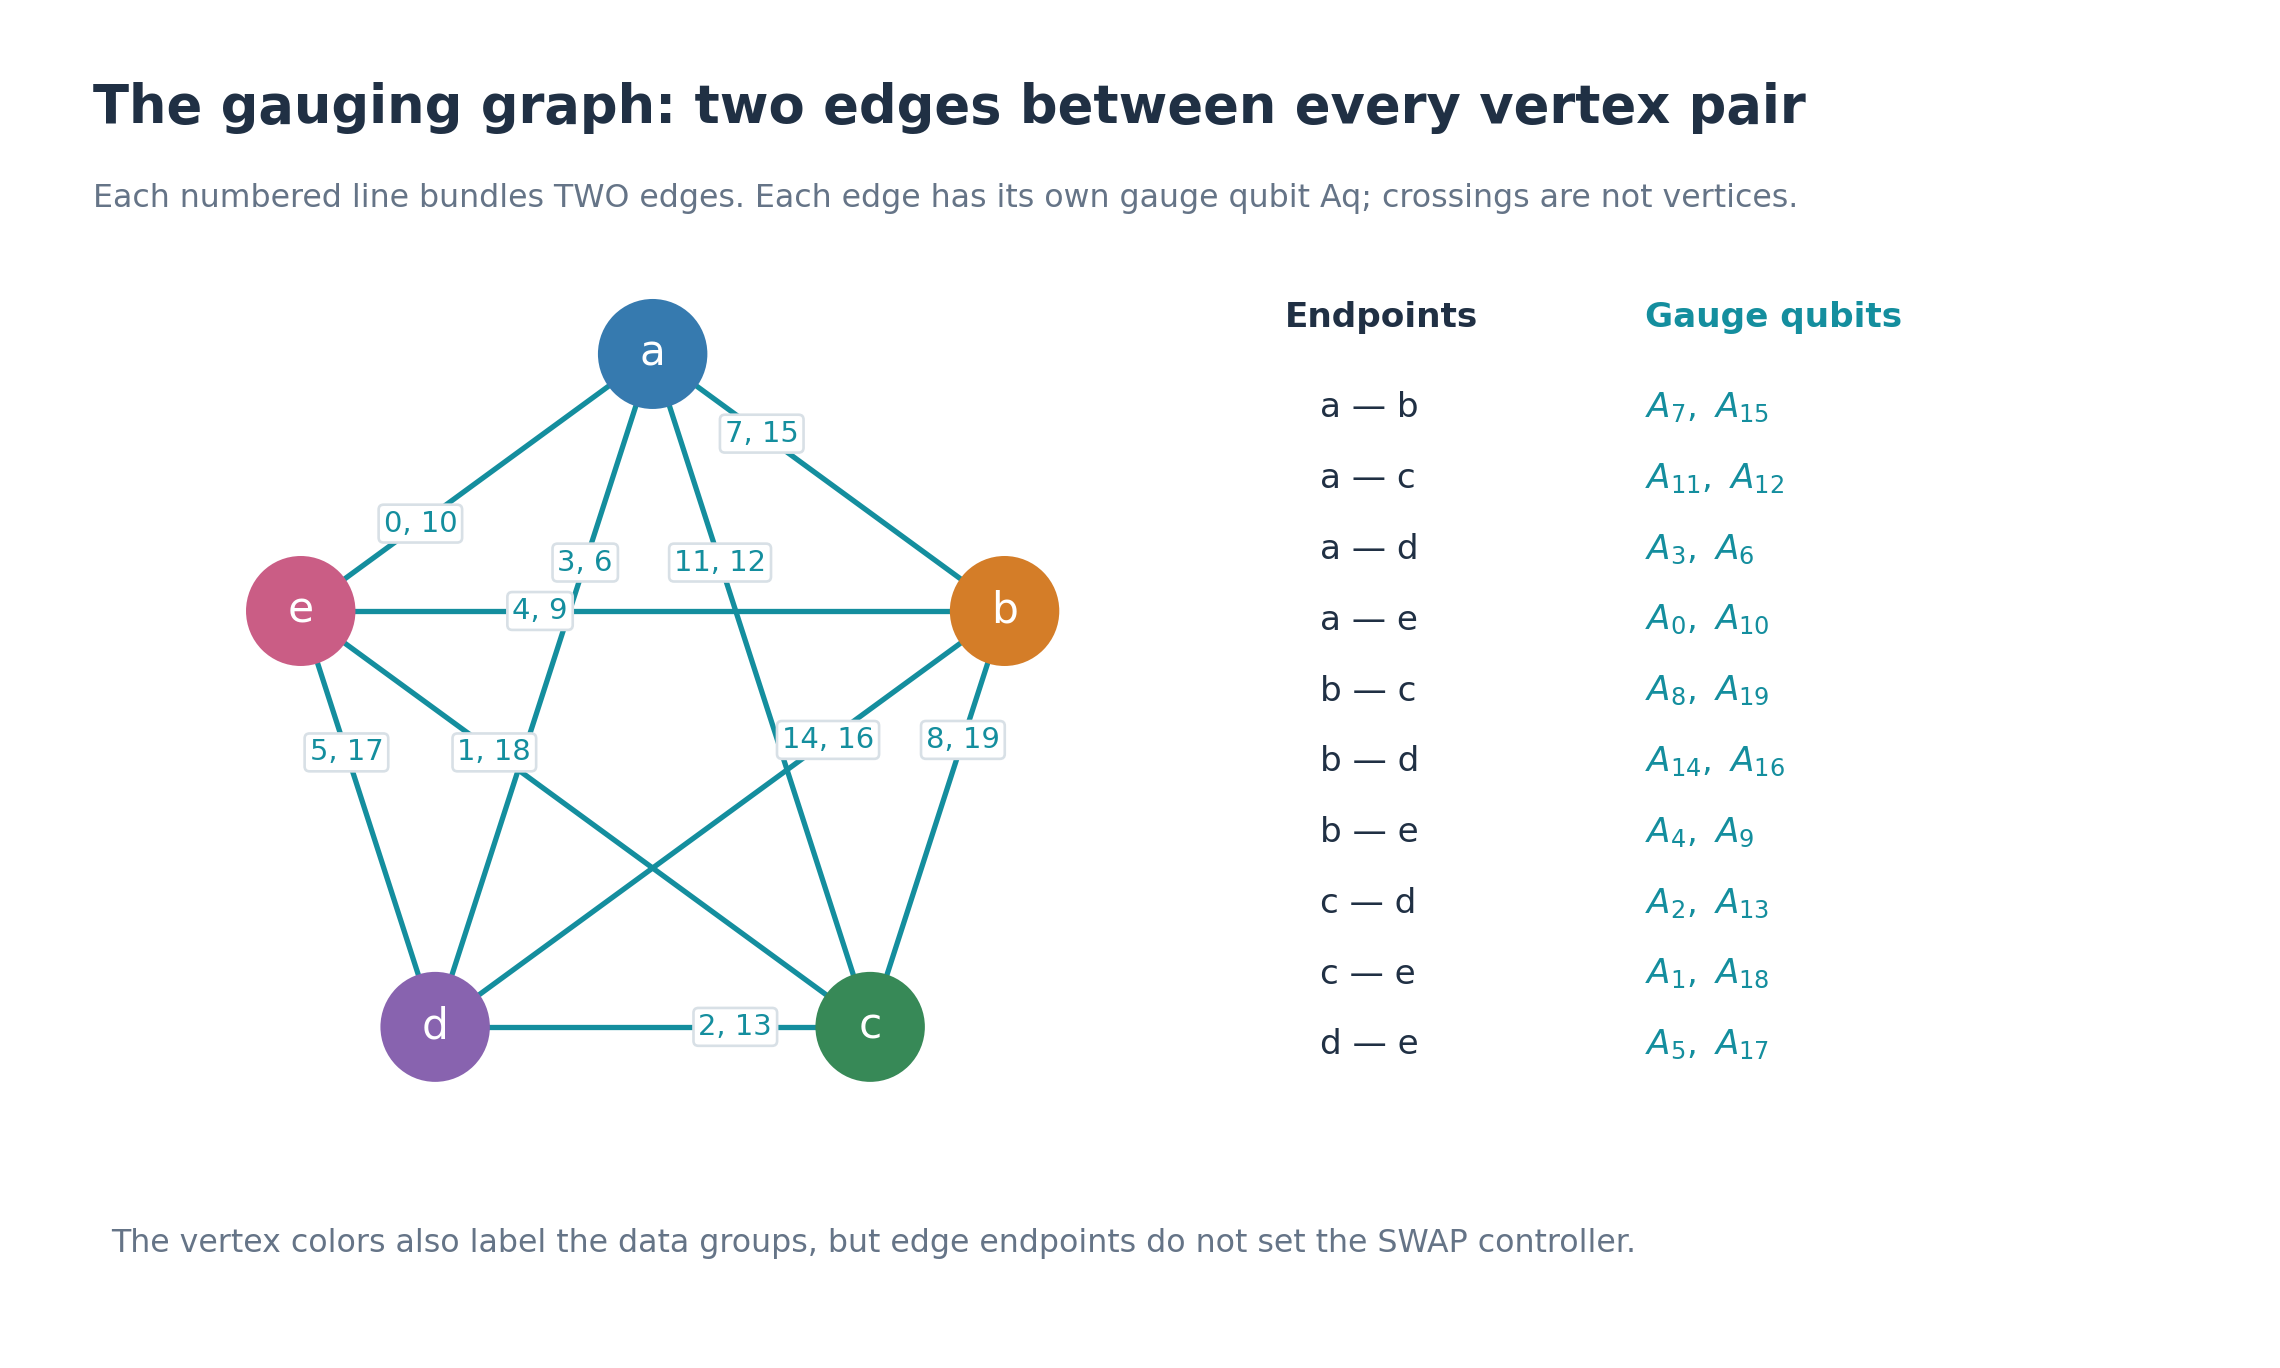
\includegraphics[width=\linewidth]{images/03-graph.png}
\captionof{figure}{The graph used throughout: each labelled line represents two edges, with one gauge qubit per edge.}
\end{minipage}\end{center}

The compiled PDF and editable LaTeX contain the same text and vector quantum circuits. This Markdown version embeds images of those circuits.

\Needspace{8\baselineskip}\section{Registers, target state, and the fault allowance}
There are twenty data qubits \(B_0,\ldots,B_{19}\), another twenty \(C_0,\ldots,C_{19}\), twenty gauge ancillas \(A_0,\ldots,A_{19}\), and five temporary vertex qubits a,b,c,d,e. Cat leaves are labelled \(\ell_j\); w is a resettable parity-measurement helper. A bar denotes a logical operator or encoded state.

Each data copy is a \([[20,2,6]]\) code. Its inner four-qubit C4 blocks have labels a:0--3, b:4--7, c:8--11, d:12--15, e:16--19. A \textbf{matched pair} means the corresponding inner blocks in B and C. For example, matched pair a contains \(B_0,\ldots,B_3,C_0,\ldots,C_3\). Two affected matched pairs can therefore contain four actual C4 blocks.

For either data copy D, the original checks are

\[
S^X_{D,s}=\prod_{q\in R_s}X_{D_q},
\qquad S^Z_{D,s}=\prod_{q\in R_s}Z_{D_q},\qquad s=0,\ldots,8.
\]

The complete supports \(R_s\) are in Appendix A. For example, \(R_0=\{0,1,2,3\}\) gives the inner XXXX and ZZZZ checks. Nine independent checks of each type specify the original code space on each copy. An encoded state is a common +1 eigenstate of these checks. Distance six means that a Pauli commuting with every check but changing the encoded information must act on at least six physical qubits. It guarantees correction of two physical-qubit errors, not two arbitrary faults in a circuit.

Prepare the inputs and define the partial and complete SWAPs by

\[
\begin{aligned}
|\psi\rangle&=|\overline{00}\rangle_B|\overline{+0}\rangle_C,\\
T_v&=\prod_{q\in J_v}\operatorname{SWAP}(B_q,C_q),\qquad
U=T_aT_bT_cT_dT_e,\qquad \Pi_+=\frac{I+U}{2}.
\end{aligned}
\]

Here \(J_v\) is the four-position inner block labelled v. The ideal state after gauging and ungauging is proportional to \(|\psi_+\rangle:=\Pi_+|\psi\rangle\). The final decoded B readout selects logical \(B_0=0\), leaving C in

\[
|\overline{M0}\rangle_C,\qquad |M\rangle=\frac{2|0\rangle+|1\rangle}{\sqrt5}.
\]

\textbf{Fault model and claim.} At most two locations fail in the entire attempt. A location is a preparation, gate, physical measurement, or single-qubit waiting interval. A faulty gate may apply an arbitrary error on its participating qubits; reports may be wrong. Classical processing is reliable. Fredkins act on their specified three qubits, or are decomposed on those same qubits. All operations are scheduled serially; unused live qubits have counted idles. Helpers are prepared inside their own gadget and reset before reuse.

The claim is that every accepted attempt within this bound has the correct \textbf{decoded} logical output. Correctable physical errors may remain. There is no new two-fault allowance at each stage.

A clean round includes all its helper preparation and idles; boundary idles belong to the following interval. Of any three complete rounds, at least one is clean. This is a fact used in the proof, not information the decoder receives.

\Needspace{8\baselineskip}\section{The measurement circuit used for every check}
\textbf{Ideal preparation.} To measure \(Q=Q_0\cdots Q_{m-1}\), with disjoint target ports, prepare one m-leaf cat. A port is one physical qubit for a Pauli factor or one data pair for a SWAP factor. The four-leaf example is

\[
|0^4\rangle\xrightarrow{H_{\ell_0},\ {\rm CNOT}_{0\to1},\ {\rm CNOT}_{1\to2},\ {\rm CNOT}_{2\to3}}
\frac{|0000\rangle+|1111\rangle}{\sqrt2}.
\]

\begin{center}\begin{minipage}{\linewidth}
\begin{center}\begin{adjustbox}{max width=\linewidth}
\begin{quantikz}[row sep={.65cm,between origins},column sep=.55cm]
\lstick{$\color{cat}\ell_0$} & \gate{\lvert0\rangle} & \gate{H} & \ctrl{1} & \qw & \qw & \qw \\
\lstick{$\color{cat}\ell_1$} & \gate{\lvert0\rangle} & \qw & \targ{} & \ctrl{1} & \qw & \qw \\
\lstick{$\color{cat}\ell_2$} & \gate{\lvert0\rangle} & \qw & \qw & \targ{} & \ctrl{1} & \qw \\
\lstick{$\color{cat}\ell_3$} & \gate{\lvert0\rangle} & \qw & \qw & \qw & \targ{} & \qw
\end{quantikz}
\end{adjustbox}\end{center}

\captionof{figure}{Raw cat preparation. A box containing zero denotes reset.}
\end{minipage}\end{center}

Extend the chain for larger m. Verify every adjacent ZZ parity three times in complete scans, using the following circuit for each pair. Reset w before each test and require every raw Z report to be zero. Reported bit zero means +1; bit one means -1.

\begin{center}\begin{minipage}{\linewidth}
\begin{center}\begin{adjustbox}{max width=\linewidth}
\begin{quantikz}[row sep={.6cm,between origins},column sep=.6cm]
\lstick{$\color{cat}\ell_j$} & \qw & \ctrl{2} & \qw & \qw & \qw \\
\lstick{$\color{cat}\ell_{j+1}$} & \qw & \qw & \ctrl{1} & \qw & \qw \\
\lstick{$\color{cat}w$} & \gate{\lvert0\rangle} & \targ{} & \targ{} & \meter{} & \rstick{$\nu_j^{(k)}$}\cw
\end{quantikz}
\end{adjustbox}\end{center}

\captionof{figure}{One adjacent-ZZ test. The parity helper w is a CNOT target.}
\end{minipage}\end{center}

Then leaf j controls \(Q_j\): CNOT for X, CZ for Z, Fredkin for SWAP. After all controlled factors, measure each leaf in X. The circuits show X measurement as H followed by a Z meter. The check bit is

\[
y=\lambda_0\oplus\cdots\oplus\lambda_{m-1}.
\]

A positive check requires \(y=0\), not every \(\lambda_j=0\). Each check uses a fresh cat. Each leaf has only one target port. Turquoise labels are gauge qubits; gold labels are cat leaves. A dot and circled plus denote CNOT, two dots denote CZ, and a quantum control with two crosses denotes Fredkin. Double wires carry classical bits. Panels sharing a cat are parts of one measurement; complete all its controlled factors before reading any of its meters.

\textbf{Example of the conditional operation.} With a possibly imperfect cat \(c_0|0^m\rangle+c_1|1^m\rangle\), coupling gives

\[
c_0|0^m\rangle|\phi\rangle+c_1|1^m\rangle Q|\phi\rangle.
\]

An actual leaf-X sign product \(r=\pm1\) leaves a data state proportional to \((c_0I+r c_1Q)|\phi\rangle\). The ideal cat and positive outcome therefore give the positive projector \((I+Q)/2\), up to a common factor for the individual leaf reports.

\textbf{Fault example and bound.} Put X on \(\ell_1\) after the first cat CNOT but before the second. After the two remaining CNOTs the leaves are in

\[
\frac{|0111\rangle+|1000\rangle}{\sqrt2}.
\]

The error spread to later leaves, but \(Z_{\ell_0}Z_{\ell_1}=-1\), so a clean verification rejects it. In general a clean ZZ scan rejects all nonuniform bit patterns and projects onto \(\operatorname{span}\{|0^m\rangle,|1^m\rangle\}\). It does not certify the relative phase: the minus cat also passes every ZZ test.

After the clean scan there are no leaf-to-leaf gates. A faulty leaf--w interaction can flip only its one leaf. X on w does not spread back to the controls; Z on w can spread phases. Thus each subsequent fault adds at most one bad leaf bit, and hence one faulty target factor. For example, X on a CNOT control leaf can produce X on its own target, but no other data target.

An operator expansion of a faulty gadget has terms

\[
D(aI+bQ).
\]

D is the local target damage: at most one target port per fault, also counting separately faulty data idles. The coefficients a,b include cat-phase faults and wrong reports. They need not give the desired projector. For instance, a minus cat with actual positive leaf parity implements \(I-Q\) instead of \(I+Q\). Repetition of complete later verification rounds must protect against this error; ZZ verification alone does not.

\Needspace{8\baselineskip}\section{Prepare the encoded B and C inputs}
\textbf{Ideal operation.} Reset all forty data qubits to zero. For each copy, measure its eighteen original checks and two logical checks, requiring positive outcomes. Execute three complete rounds on B, then three on C:

\[
\begin{aligned}
\mathcal F_B&=(S^X_{B,0:8},S^Z_{B,0:8},\overline Z^B_0,\overline Z^B_1),\\
\mathcal F_C&=(S^X_{C,0:8},S^Z_{C,0:8},\overline X^C_0,\overline Z^C_1).
\end{aligned}
\]

Here \(0{:}8\) means the nine checks in increasing s order. The logical supports are listed in Appendix A. The positive projector for a full B source round is \(|\overline{00}\rangle\langle\overline{00}|\); for C it is \(|\overline{+0}\rangle\langle\overline{+0}|\).

\begin{center}\begin{minipage}{\linewidth}
\par\noindent\begin{minipage}[t]{.485\linewidth}\centering\small\textbf{XXXX check}
\begin{center}\begin{adjustbox}{max width=\linewidth}
\begin{quantikz}[row sep={.46cm,between origins},column sep=.22cm]
\lstick{$\color{cat}\ell_{0}$} & \ctrl{1} & \qw & \qw & \qw & \gate{H} & \meter{} & \rstick{$\lambda_{0}$}\cw \\
\lstick{$\color{groupa}D_0$} & \targ{} & \qw & \qw & \qw & \qw & \qw & \qw \\
\lstick{$\color{cat}\ell_{1}$} & \qw & \ctrl{1} & \qw & \qw & \gate{H} & \meter{} & \rstick{$\lambda_{1}$}\cw \\
\lstick{$\color{groupa}D_1$} & \qw & \targ{} & \qw & \qw & \qw & \qw & \qw \\
\lstick{$\color{cat}\ell_{2}$} & \qw & \qw & \ctrl{1} & \qw & \gate{H} & \meter{} & \rstick{$\lambda_{2}$}\cw \\
\lstick{$\color{groupa}D_2$} & \qw & \qw & \targ{} & \qw & \qw & \qw & \qw \\
\lstick{$\color{cat}\ell_{3}$} & \qw & \qw & \qw & \ctrl{1} & \gate{H} & \meter{} & \rstick{$\lambda_{3}$}\cw \\
\lstick{$\color{groupa}D_3$} & \qw & \qw & \qw & \targ{} & \qw & \qw & \qw
\end{quantikz}
\end{adjustbox}\end{center}
\end{minipage}\hfill\begin{minipage}[t]{.485\linewidth}\centering\small\textbf{ZZZZ check}
\begin{center}\begin{adjustbox}{max width=\linewidth}
\begin{quantikz}[row sep={.46cm,between origins},column sep=.22cm]
\lstick{$\color{cat}\ell_{0}$} & \ctrl{1} & \qw & \qw & \qw & \gate{H} & \meter{} & \rstick{$\lambda_{0}$}\cw \\
\lstick{$\color{groupa}D_0$} & \control{} & \qw & \qw & \qw & \qw & \qw & \qw \\
\lstick{$\color{cat}\ell_{1}$} & \qw & \ctrl{1} & \qw & \qw & \gate{H} & \meter{} & \rstick{$\lambda_{1}$}\cw \\
\lstick{$\color{groupa}D_1$} & \qw & \control{} & \qw & \qw & \qw & \qw & \qw \\
\lstick{$\color{cat}\ell_{2}$} & \qw & \qw & \ctrl{1} & \qw & \gate{H} & \meter{} & \rstick{$\lambda_{2}$}\cw \\
\lstick{$\color{groupa}D_2$} & \qw & \qw & \control{} & \qw & \qw & \qw & \qw \\
\lstick{$\color{cat}\ell_{3}$} & \qw & \qw & \qw & \ctrl{1} & \gate{H} & \meter{} & \rstick{$\lambda_{3}$}\cw \\
\lstick{$\color{groupa}D_3$} & \qw & \qw & \qw & \control{} & \qw & \qw & \qw
\end{quantikz}
\end{adjustbox}\end{center}
\end{minipage}\par

\captionof{figure}{Physical circuits for inner XXXX and ZZZZ checks; D denotes either data copy.}
\end{minipage}\end{center}

Replace the four targets by \(R_s\) for another code check, or by a logical support for an input logical check. Use one shared cat per panel, with six leaves for a logical check and eight for an upper check.

\textbf{Fault example.} After a correct source state has been prepared, \(X_{B_0}\) makes its inner ZZZZ outcome negative. A later clean positive source round rejects this component. A fault in raw preparation can cause a more complicated state; the clean full round projects onto the unique intended source state or rejects it.

Later measurement faults leave local damage. If F is an existing error, Q a measured source stabilizer, and \(|\sigma\rangle\) the intended source,

\[
(aI+bQ)F|\sigma\rangle=(aF+bQFQ)|\sigma\rangle,
\qquad Q|\sigma\rangle=|\sigma\rangle.
\]

Pauli conjugation by Q does not enlarge F's support. A gadget's additional D contributes only its faulty targets. Thus residual source errors have at most one physical source-qubit error per fault after its clean round. B waiting while C and the graph are prepared is included in this count.

\Needspace{8\baselineskip}\section{Prepare and verify the graph resource}
\textbf{Ideal operation.} Reset the five vertices and twenty A qubits to zero. Apply H to each vertex. For every edge q with endpoints \(u_q,v_q\), apply CNOT from \(u_q\) to \(A_q\), then from \(v_q\) to \(A_q\). Use increasing q and alphabetic endpoint order. There are forty CNOTs.

The state is

\[
|\Gamma\rangle_{VA}=\frac1{\sqrt{32}}\sum_{t\in\{0,1\}^5}
|t\rangle_V|p(t)\rangle_A,\qquad p(t)_q=t_{u_q}\oplus t_{v_q}.
\]

\begin{center}\begin{minipage}{\linewidth}
\begin{center}\begin{adjustbox}{max width=\linewidth}
\begin{quantikz}[row sep={.65cm,between origins},column sep=.43cm]
\lstick{$\color{groupa}a$} & \gate{\lvert0\rangle} & \gate{H} & \ctrl{3} & \qw & \qw & \qw & \qw \\
\lstick{$\color{groupc}c$} & \gate{\lvert0\rangle} & \gate{H} & \qw & \qw & \ctrl{3} & \qw & \qw \\
\lstick{$\color{groupe}e$} & \gate{\lvert0\rangle} & \gate{H} & \qw & \ctrl{1} & \qw & \ctrl{2} & \qw \\
\lstick{$\color{gauge}A_0$} & \gate{\lvert0\rangle} & \qw & \targ{} & \targ{} & \qw & \qw & \qw \\
\lstick{$\color{gauge}A_1$} & \gate{\lvert0\rangle} & \qw & \qw & \qw & \targ{} & \targ{} & \qw
\end{quantikz}
\end{adjustbox}\end{center}

\captionof{figure}{The resource gates for edges 0 (a--e) and 1 (c--e).}
\end{minipage}\end{center}

The subscript V denotes the five temporary vertices. The twenty-bit string \(p(t)\) lists the actual computational-basis values of A. For example, \(t=00000\) and \(t=11111\) both give \(p(t)=0^{20}\): each edge receives either no flips or two flips. Both terms are present in the superposition, together with the other thirty terms.

Verify the 25 checks in the order shown below, in three complete positive rounds. They specify \(|\Gamma\rangle\) uniquely:

\[
K_v=X_v\prod_{q\in E_v}X_{A_q},\qquad
K_q=Z_{u_q}Z_{A_q}Z_{v_q},\qquad
(K_a,\ldots,K_e,K_0,\ldots,K_{19}).
\]

Here \(E_v\) is the eight-edge star incident on v. In particular, \(E_a=\{0,3,6,7,10,11,12,15\}\). Each resource-edge check has three ports; each vertex check has nine, including the still-live vertex.

\begin{center}\begin{minipage}{\linewidth}
\begin{center}\begin{adjustbox}{max width=\linewidth}
\begin{quantikz}[row sep={.46cm,between origins},column sep=.22cm]
\lstick{$\color{cat}\ell_{0}$} & \ctrl{1} & \qw & \qw & \gate{H} & \meter{} & \rstick{$\lambda_{0}$}\cw \\
\lstick{$\color{groupc}c$} & \control{} & \qw & \qw & \qw & \qw & \qw \\
\lstick{$\color{cat}\ell_{1}$} & \qw & \ctrl{1} & \qw & \gate{H} & \meter{} & \rstick{$\lambda_{1}$}\cw \\
\lstick{$\color{gauge}A_1$} & \qw & \control{} & \qw & \qw & \qw & \qw \\
\lstick{$\color{cat}\ell_{2}$} & \qw & \qw & \ctrl{1} & \gate{H} & \meter{} & \rstick{$\lambda_{2}$}\cw \\
\lstick{$\color{groupe}e$} & \qw & \qw & \control{} & \qw & \qw & \qw
\end{quantikz}
\end{adjustbox}\end{center}

\captionof{figure}{One edge check: \(K_1\) has targets c, \(A_1\), e.}
\end{minipage}\end{center}

\begin{center}\begin{minipage}{\linewidth}
\par\noindent\begin{minipage}[t]{.485\linewidth}\centering\small\textbf{Leaves 0--4}
\begin{center}\begin{adjustbox}{max width=\linewidth}
\begin{quantikz}[row sep={.46cm,between origins},column sep=.22cm]
\lstick{$\color{cat}\ell_{0}$} & \ctrl{1} & \qw & \qw & \qw & \qw & \gate{H} & \meter{} & \rstick{$\lambda_{0}$}\cw \\
\lstick{$\color{groupa}a$} & \targ{} & \qw & \qw & \qw & \qw & \qw & \qw & \qw \\
\lstick{$\color{cat}\ell_{1}$} & \qw & \ctrl{1} & \qw & \qw & \qw & \gate{H} & \meter{} & \rstick{$\lambda_{1}$}\cw \\
\lstick{$\color{gauge}A_{0}$} & \qw & \targ{} & \qw & \qw & \qw & \qw & \qw & \qw \\
\lstick{$\color{cat}\ell_{2}$} & \qw & \qw & \ctrl{1} & \qw & \qw & \gate{H} & \meter{} & \rstick{$\lambda_{2}$}\cw \\
\lstick{$\color{gauge}A_{3}$} & \qw & \qw & \targ{} & \qw & \qw & \qw & \qw & \qw \\
\lstick{$\color{cat}\ell_{3}$} & \qw & \qw & \qw & \ctrl{1} & \qw & \gate{H} & \meter{} & \rstick{$\lambda_{3}$}\cw \\
\lstick{$\color{gauge}A_{6}$} & \qw & \qw & \qw & \targ{} & \qw & \qw & \qw & \qw \\
\lstick{$\color{cat}\ell_{4}$} & \qw & \qw & \qw & \qw & \ctrl{1} & \gate{H} & \meter{} & \rstick{$\lambda_{4}$}\cw \\
\lstick{$\color{gauge}A_{7}$} & \qw & \qw & \qw & \qw & \targ{} & \qw & \qw & \qw
\end{quantikz}
\end{adjustbox}\end{center}
\end{minipage}\hfill\begin{minipage}[t]{.485\linewidth}\centering\small\textbf{Leaves 5--8}
\begin{center}\begin{adjustbox}{max width=\linewidth}
\begin{quantikz}[row sep={.46cm,between origins},column sep=.22cm]
\lstick{$\color{cat}\ell_{5}$} & \ctrl{1} & \qw & \qw & \qw & \gate{H} & \meter{} & \rstick{$\lambda_{5}$}\cw \\
\lstick{$\color{gauge}A_{10}$} & \targ{} & \qw & \qw & \qw & \qw & \qw & \qw \\
\lstick{$\color{cat}\ell_{6}$} & \qw & \ctrl{1} & \qw & \qw & \gate{H} & \meter{} & \rstick{$\lambda_{6}$}\cw \\
\lstick{$\color{gauge}A_{11}$} & \qw & \targ{} & \qw & \qw & \qw & \qw & \qw \\
\lstick{$\color{cat}\ell_{7}$} & \qw & \qw & \ctrl{1} & \qw & \gate{H} & \meter{} & \rstick{$\lambda_{7}$}\cw \\
\lstick{$\color{gauge}A_{12}$} & \qw & \qw & \targ{} & \qw & \qw & \qw & \qw \\
\lstick{$\color{cat}\ell_{8}$} & \qw & \qw & \qw & \ctrl{1} & \gate{H} & \meter{} & \rstick{$\lambda_{8}$}\cw \\
\lstick{$\color{gauge}A_{15}$} & \qw & \qw & \qw & \targ{} & \qw & \qw & \qw
\end{quantikz}
\end{adjustbox}\end{center}
\end{minipage}\par

\captionof{figure}{All nine ports of \(K_a\), split across two panels sharing one cat.}
\end{minipage}\end{center}

\textbf{Fault example.} Let an X fault occur on a after its CNOTs to \(A_0,A_3,A_6\), but before its five remaining CNOTs. Propagation through those remaining gates leaves

\[
X_aX_{A_7}X_{A_{10}}X_{A_{11}}X_{A_{12}}X_{A_{15}}|\Gamma\rangle
=X_{A_0}X_{A_3}X_{A_6}|\Gamma\rangle.
\]

The equality uses \(K_a|\Gamma\rangle=|\Gamma\rangle\). One raw fault can therefore produce more than one bad gauge bit. Clean verification rejects this component: \(K_0,K_3,K_6\) are negative.

A clean complete source round projects any accepted input onto \(|\Gamma\rangle\). Later Pauli-check gadgets preserve local residual support by the same calculation as in Section 3. A remaining vertex error can affect one matched pair during enrichment; an A bit error affects only its one gauge position. Raw graph preparation is not being assumed fault tolerant by itself.

\Needspace{8\baselineskip}\section{Apply the twenty enrichment Fredkins}
\textbf{Ideal operation.} Vertex v controls the four SWAPs with physical labels in \(J_v\). With \(V_t=\prod_vT_v^{t_v}\),

\[
|\Gamma\rangle|\psi\rangle
\longmapsto
\frac1{\sqrt{32}}\sum_t |t\rangle_V|p(t)\rangle_A V_t|\psi\rangle.
\]

\begin{center}\begin{minipage}{\linewidth}
\begin{center}\begin{adjustbox}{max width=\linewidth}
\begin{quantikz}[row sep={.58cm,between origins},column sep=.55cm]
\lstick{$\color{groupa}a$} & \ctrl{1} & \ctrl{3} & \ctrl{5} & \ctrl{7} & \gate{H} & \meter{} & \rstick{$b_a$}\cw \\
\lstick{$\color{groupa}B_0$} & \swap{1} & \qw & \qw & \qw & \qw & \qw & \qw \\
\lstick{$\color{groupa}C_0$} & \targX{} & \qw & \qw & \qw & \qw & \qw & \qw \\
\lstick{$\color{groupa}B_1$} & \qw & \swap{1} & \qw & \qw & \qw & \qw & \qw \\
\lstick{$\color{groupa}C_1$} & \qw & \targX{} & \qw & \qw & \qw & \qw & \qw \\
\lstick{$\color{groupa}B_2$} & \qw & \qw & \swap{1} & \qw & \qw & \qw & \qw \\
\lstick{$\color{groupa}C_2$} & \qw & \qw & \targX{} & \qw & \qw & \qw & \qw \\
\lstick{$\color{groupa}B_3$} & \qw & \qw & \qw & \swap{1} & \qw & \qw & \qw \\
\lstick{$\color{groupa}C_3$} & \qw & \qw & \qw & \targX{} & \qw & \qw & \qw
\end{quantikz}
\end{adjustbox}\end{center}

\captionof{figure}{Four Fredkins controlled by a. Complete all twenty Fredkins before any vertex meter is read.}
\end{minipage}\end{center}

The controller assignment is a:0--3, b:4--7, c:8--11, d:12--15, e:16--19. It differs from the edge endpoints. For example, \(A_1\) has endpoints c,e, while the pair \(B_1,C_1\) is controlled by a.

\textbf{Example of the superposition.} The vertex strings \(t=01000\) and \(\bar t=10111\) give the same A string: ones on the eight edges touching b, zeros elsewhere. Their data states after enrichment are, respectively,

\[
T_b|\psi\rangle,\qquad T_aT_cT_dT_e|\psi\rangle=T_bU|\psi\rangle.
\]

These are two components passing through one circuit. The bar flips all five vertex bits; it does not denote logical encoding.

\textbf{Fault example.} An X fault on a after its first Fredkin is propagated through the remaining three as an X on a times ordinary SWAPs on pairs 1,2,3. For one controlled-SWAP gate F,

\[
F X_a F=X_a\,\operatorname{SWAP}(B_q,C_q).
\]

Several data pairs can therefore be damaged, but all are in matched pair a. A faulty Fredkin can also damage its own data targets; they belong to the same matched pair as its controller. Existing data errors may exchange B/C positions, but not matched-pair labels. This is why one controller is assigned to only one matched pair.

\Needspace{8\baselineskip}\section{Read the vertices and apply the ancilla-Z corrections}
\textbf{Ideal operation.} Measure a,b,c,d,e in X, obtaining reported bits \(b_a,\ldots,b_e\). Require even parity. Then apply

\[
b_a\oplus b_b\oplus b_c\oplus b_d\oplus b_e=0,\qquad
F_b=Z_{A_7}^{b_b}Z_{A_{11}}^{b_c}Z_{A_3}^{b_d}Z_{A_0}^{b_e}.
\]

These are physical Z gates controlled by classical reports. The root is a; the four chosen edges join a to b,c,d,e. Reset the measured vertices for helper reuse.

\begin{center}\begin{minipage}{\linewidth}
\par\noindent\begin{minipage}[t]{.485\linewidth}\centering\small\textbf{$b_b$ selects $Z_{A_7}$}
\begin{center}\begin{adjustbox}{max width=\linewidth}
\begin{quantikz}[row sep={.65cm,between origins},column sep=.65cm]
\lstick{$\color{groupb}b_b$} & \cwbend{1} & \cw \\
\lstick{$\color{gauge}A_{7}$} & \gate{Z} & \qw
\end{quantikz}
\end{adjustbox}\end{center}
\end{minipage}\hfill\begin{minipage}[t]{.485\linewidth}\centering\small\textbf{$b_c$ selects $Z_{A_{11}}$}
\begin{center}\begin{adjustbox}{max width=\linewidth}
\begin{quantikz}[row sep={.65cm,between origins},column sep=.65cm]
\lstick{$\color{groupc}b_c$} & \cwbend{1} & \cw \\
\lstick{$\color{gauge}A_{11}$} & \gate{Z} & \qw
\end{quantikz}
\end{adjustbox}\end{center}
\end{minipage}\par
\vspace{3mm}
\par\noindent\begin{minipage}[t]{.485\linewidth}\centering\small\textbf{$b_d$ selects $Z_{A_3}$}
\begin{center}\begin{adjustbox}{max width=\linewidth}
\begin{quantikz}[row sep={.65cm,between origins},column sep=.65cm]
\lstick{$\color{groupd}b_d$} & \cwbend{1} & \cw \\
\lstick{$\color{gauge}A_{3}$} & \gate{Z} & \qw
\end{quantikz}
\end{adjustbox}\end{center}
\end{minipage}\hfill\begin{minipage}[t]{.485\linewidth}\centering\small\textbf{$b_e$ selects $Z_{A_0}$}
\begin{center}\begin{adjustbox}{max width=\linewidth}
\begin{quantikz}[row sep={.65cm,between origins},column sep=.65cm]
\lstick{$\color{groupe}b_e$} & \cwbend{1} & \cw \\
\lstick{$\color{gauge}A_{0}$} & \gate{Z} & \qw
\end{quantikz}
\end{adjustbox}\end{center}
\end{minipage}\par

\captionof{figure}{The four classical report-to-Z corrections. Double wires carry measured bits.}
\end{minipage}\end{center}

For example, \(b_b=b_d=1\) and the other three bits zero is accepted. Apply \(Z_{A_7}Z_{A_3}\). Before this correction, the amplitude of a vertex term t contains \((-1)^{t_b+t_d}\). The Z gates multiply it by \((-1)^{(t_a+t_b)+(t_a+t_d)}\), cancelling the sign.

For any accepted b, pairing t with its complement gives the corrected unnormalized branch state

\[
\frac1{16}\sum_{t:t_a=0}|p(t)\rangle_A V_t|\psi_+\rangle,
\qquad |\psi_+\rangle=\frac{I+U}{2}|\psi\rangle.
\]

The two computational components contributed \(V_t|\psi\rangle\) and \(V_tU|\psi\rangle\). X readout combines them; F\_b removes their unwanted individual signs. The common relative plus sign implements the positive SWAP projection.

For subsequent equations define the reference vectors

\[
|\psi_\pm\rangle=\frac{I\pm U}{2}|\psi\rangle,\qquad
|\Phi_\pm\rangle=\frac14\sum_{t:t_a=0}|p(t)\rangle_A V_t|\psi_\pm\rangle.
\]

They may be unnormalized; the corrected ideal branch above is \(|\Phi_+\rangle/4\). U acts only on the data and commutes with every \(V_t\), hence \(U|\Phi_\pm\rangle=\pm|\Phi_\pm\rangle\).

\textbf{Fault example.} A Z fault on a just before its X measurement multiplies the t component by \((-1)^{t_a}\). For reported b=00000, the two terms t and its complement now combine with a minus sign: the branch can contain \(|\Phi_-\rangle\) instead of \(|\Phi_+\rangle\). This does not require many damaged data qubits. The measured SWAP projection itself is wrong. The checks in the next sections are needed to detect it; the spatial error bound alone cannot do so.

More general wrong amplitudes can depend on \(t_b,t_c,t_d,t_e\) when the representative has \(t_a=0\). Any function of these four bits is a linear combination of the sixteen products of their signs \((-1)^{t_v}\). On A, those signs are supplied by \(Z_{A_7},Z_{A_{11}},Z_{A_3},Z_{A_0}\), respectively, since the four tree-edge bits equal \(t_b,t_c,t_d,t_e\). Thus those amplitude errors can be expanded as gauge-Z operators. Including the bounded gauge-bit and local data errors, the state before a clean round is a sum of terms \(F_A E|\Phi_\pm\rangle\), where \(F_A\) acts only on A. Its X part has weight at most the number of faults; its Z part can be unrestricted. E occupies at most one new matched-pair label per fault. This accounts for unequal or missing contributions rather than assuming they already combine correctly.

\Needspace{8\baselineskip}\section{While gauged: measure the eighteen paired checks}
\textbf{Ideal operation.} Measure, in order, the nine X products and nine Z products

\[
N_s^P=S^P_{B,s}S^P_{C,s},\qquad s=0,\ldots,8,\quad P=X,Z.
\]

Use one cat across both copies for each check, with B targets first. All leaf-X parities must be zero. Both \(|\Phi_+\rangle\) and \(|\Phi_-\rangle\) satisfy these paired checks: the original inputs do, and matched factors \(P_{B_q}P_{C_q}\) commute with SWAP.

\begin{center}\begin{minipage}{\linewidth}
\par\noindent\begin{minipage}[t]{.485\linewidth}\centering\small\textbf{B ports: leaves 0--3}
\begin{center}\begin{adjustbox}{max width=\linewidth}
\begin{quantikz}[row sep={.46cm,between origins},column sep=.22cm]
\lstick{$\color{cat}\ell_{0}$} & \ctrl{1} & \qw & \qw & \qw & \gate{H} & \meter{} & \rstick{$\lambda_{0}$}\cw \\
\lstick{$\color{groupa}B_0$} & \targ{} & \qw & \qw & \qw & \qw & \qw & \qw \\
\lstick{$\color{cat}\ell_{1}$} & \qw & \ctrl{1} & \qw & \qw & \gate{H} & \meter{} & \rstick{$\lambda_{1}$}\cw \\
\lstick{$\color{groupa}B_1$} & \qw & \targ{} & \qw & \qw & \qw & \qw & \qw \\
\lstick{$\color{cat}\ell_{2}$} & \qw & \qw & \ctrl{1} & \qw & \gate{H} & \meter{} & \rstick{$\lambda_{2}$}\cw \\
\lstick{$\color{groupa}B_2$} & \qw & \qw & \targ{} & \qw & \qw & \qw & \qw \\
\lstick{$\color{cat}\ell_{3}$} & \qw & \qw & \qw & \ctrl{1} & \gate{H} & \meter{} & \rstick{$\lambda_{3}$}\cw \\
\lstick{$\color{groupa}B_3$} & \qw & \qw & \qw & \targ{} & \qw & \qw & \qw
\end{quantikz}
\end{adjustbox}\end{center}
\end{minipage}\hfill\begin{minipage}[t]{.485\linewidth}\centering\small\textbf{C ports: leaves 4--7}
\begin{center}\begin{adjustbox}{max width=\linewidth}
\begin{quantikz}[row sep={.46cm,between origins},column sep=.22cm]
\lstick{$\color{cat}\ell_{4}$} & \ctrl{1} & \qw & \qw & \qw & \gate{H} & \meter{} & \rstick{$\lambda_{4}$}\cw \\
\lstick{$\color{groupa}C_0$} & \targ{} & \qw & \qw & \qw & \qw & \qw & \qw \\
\lstick{$\color{cat}\ell_{5}$} & \qw & \ctrl{1} & \qw & \qw & \gate{H} & \meter{} & \rstick{$\lambda_{5}$}\cw \\
\lstick{$\color{groupa}C_1$} & \qw & \targ{} & \qw & \qw & \qw & \qw & \qw \\
\lstick{$\color{cat}\ell_{6}$} & \qw & \qw & \ctrl{1} & \qw & \gate{H} & \meter{} & \rstick{$\lambda_{6}$}\cw \\
\lstick{$\color{groupa}C_2$} & \qw & \qw & \targ{} & \qw & \qw & \qw & \qw \\
\lstick{$\color{cat}\ell_{7}$} & \qw & \qw & \qw & \ctrl{1} & \gate{H} & \meter{} & \rstick{$\lambda_{7}$}\cw \\
\lstick{$\color{groupa}C_3$} & \qw & \qw & \qw & \targ{} & \qw & \qw & \qw
\end{quantikz}
\end{adjustbox}\end{center}
\end{minipage}\par

\captionof{figure}{One eight-leaf cat for \(N_0^X\). The panels yield one combined parity.}
\end{minipage}\end{center}

For an eight-position upper support \(R_s\), the cat has sixteen leaves. Z products use CZ gates instead of CNOTs. Individual B and C stabilizers are not measured separately at this stage.

\textbf{Error examples.} \(X_{B_0}\) flips the paired inner-Z check and is rejected by a clean positive measurement. In contrast, keep the following example through the rest of the protocol:

\[
E=X_{B_0}X_{C_1}X_{C_2}X_{C_3}.
\]

It gives one minus sign on B and three on C, so their paired inner-Z product stays positive. In fact it passes every paired check. Write its one-copy patterns as \(P=X_0,\ R=X_1X_2X_3\). Then

\[
P^\dagger R=X_0X_1X_2X_3=S,\qquad
E=(P_BP_C)S_C.
\]

Here S is the inner XXXX stabilizer. \(P_C\) is the same pattern as P applied to C; it cancels an extra \(X_{C_0}\) in \(S_C\). P on B has not been changed. The dagger is the inverse of P.

\textbf{Why this is enough for general surviving errors.} The code has the following two-group property: a Pauli on at most two inner C4 blocks of one copy, commuting with all its checks, is a stabilizer up to phase. To see it, separate its X and Z parts, using \(Y=iXZ\). Inner checks force an even number of each per block. Multiplying by inner XXXX or ZZZZ removes four equal factors, leaving each part at weight at most four. Since every generator contains only X or only Z, both parts individually commute with all checks. Distance six excludes a nontrivial logical action for either part.

For a general two-matched-pair Pauli \(E=P_BR_C\), passing paired checks means P and R have the same commutation sign with every original check. Thus \(P^\dagger R\) is an undetected one-copy Pauli on at most two inner blocks, and the property just proved gives \(P^\dagger R=S\). Consequently \(E=(P_BP_C)S_C\), up to phase.

On states passing paired checks, \(S_BS_C=+1\), hence S on B and C act identically. The factor \(P_BP_C\) is unchanged by exchanging copies. It follows that

\[
UE|\chi\rangle=EU|\chi\rangle
\quad\text{if all paired checks on }|\chi\rangle\text{ are positive}.
\]

For the worked example this can be checked without the general argument:

\[
UEU=X_{C_0}X_{B_1}X_{B_2}X_{B_3}=E N_0^X.
\]

On paired-positive states, E and its exchanged version therefore act identically. A surviving error cannot convert a negative U eigenvalue to a positive one. Phase and bit operators on A commute with U and do not change this conclusion.

\Needspace{8\baselineskip}\section{While gauged: measure the sixteen cycle checks}
\textbf{Ideal operation.} For each cycle support \(\eta\), measure \(L_\eta=\prod_{q\in\eta}Z_{A_q}\), with one fresh cat and CZ couplings. The ideal strings \(p(t)\) give +1: along a closed cycle, each vertex bit occurs twice in the XOR of the edge bits.

\begin{center}\begin{minipage}{\linewidth}
\par\noindent\begin{minipage}[t]{.485\linewidth}\centering\small\textbf{Parallel edges 7,15}
\begin{center}\begin{adjustbox}{max width=\linewidth}
\begin{quantikz}[row sep={.46cm,between origins},column sep=.22cm]
\lstick{$\color{cat}\ell_{0}$} & \ctrl{1} & \qw & \gate{H} & \meter{} & \rstick{$\lambda_{0}$}\cw \\
\lstick{$\color{gauge}A_7$} & \control{} & \qw & \qw & \qw & \qw \\
\lstick{$\color{cat}\ell_{1}$} & \qw & \ctrl{1} & \gate{H} & \meter{} & \rstick{$\lambda_{1}$}\cw \\
\lstick{$\color{gauge}A_{15}$} & \qw & \control{} & \qw & \qw & \qw
\end{quantikz}
\end{adjustbox}\end{center}
\end{minipage}\hfill\begin{minipage}[t]{.485\linewidth}\centering\small\textbf{Triangle 7,8,11}
\begin{center}\begin{adjustbox}{max width=\linewidth}
\begin{quantikz}[row sep={.46cm,between origins},column sep=.22cm]
\lstick{$\color{cat}\ell_{0}$} & \ctrl{1} & \qw & \qw & \gate{H} & \meter{} & \rstick{$\lambda_{0}$}\cw \\
\lstick{$\color{gauge}A_7$} & \control{} & \qw & \qw & \qw & \qw & \qw \\
\lstick{$\color{cat}\ell_{1}$} & \qw & \ctrl{1} & \qw & \gate{H} & \meter{} & \rstick{$\lambda_{1}$}\cw \\
\lstick{$\color{gauge}A_8$} & \qw & \control{} & \qw & \qw & \qw & \qw \\
\lstick{$\color{cat}\ell_{2}$} & \qw & \qw & \ctrl{1} & \gate{H} & \meter{} & \rstick{$\lambda_{2}$}\cw \\
\lstick{$\color{gauge}A_{11}$} & \qw & \qw & \control{} & \qw & \qw & \qw
\end{quantikz}
\end{adjustbox}\end{center}
\end{minipage}\par

\captionof{figure}{Parallel-edge and triangle cycle-check circuits.}
\end{minipage}\end{center}

The ordered supports are

\[
\begin{aligned}
&(7,15),(11,12),(3,6),(0,10),(8,19),\\
&(14,16),(4,9),(2,13),(1,18),(5,17),\\
&(7,8,11),(7,14,3),(7,4,0),\\
&(11,2,3),(11,1,0),(3,5,0).
\end{aligned}
\]

\textbf{Fault example.} \(X_{A_7}\) changes the sign of \(L_{(7,15)}=Z_{A_7}Z_{A_{15}}\), so a clean positive cycle check rejects it. A gauge Z error does not change this outcome; cycle checks certify bit consistency, not all possible phase errors.

These sixteen independent constraints characterize the sixteen valid strings \(p(t)\). Different such strings are separated by at least eight positions, as proved in Section 10. Thus a nonzero X pattern of weight one or two cannot move one valid string to another; a clean complete cycle measurement rejects those terms. Faulty cycle gadgets touch only individual A ports, while their cat-phase uncertainty is allowed in the coefficients of \(aI+bL_\eta\).

\Needspace{8\baselineskip}\section{While gauged: Gauss checks protect the SWAP projection}
\textbf{Ideal operation.} For v=a,b,c,d,e, measure

\[
G_v=\left(\prod_{q\in E_v}X_{A_q}\right)T_v.
\]

Use one twelve-leaf cat: eight CNOT ports to the gauge star, then four Fredkin ports to the corresponding data pairs. Measure all twelve leaves in X only after all controlled factors. Require their one parity to be zero.

\begin{center}\begin{minipage}{\linewidth}
\par\noindent\begin{minipage}[t]{.485\linewidth}\centering\small\textbf{Gauge ports 0--3}
\begin{center}\begin{adjustbox}{max width=\linewidth}
\begin{quantikz}[row sep={.46cm,between origins},column sep=.22cm]
\lstick{$\color{cat}\ell_{0}$} & \ctrl{1} & \qw & \qw & \qw & \gate{H} & \meter{} & \rstick{$\lambda_{0}$}\cw \\
\lstick{$\color{gauge}A_{0}$} & \targ{} & \qw & \qw & \qw & \qw & \qw & \qw \\
\lstick{$\color{cat}\ell_{1}$} & \qw & \ctrl{1} & \qw & \qw & \gate{H} & \meter{} & \rstick{$\lambda_{1}$}\cw \\
\lstick{$\color{gauge}A_{3}$} & \qw & \targ{} & \qw & \qw & \qw & \qw & \qw \\
\lstick{$\color{cat}\ell_{2}$} & \qw & \qw & \ctrl{1} & \qw & \gate{H} & \meter{} & \rstick{$\lambda_{2}$}\cw \\
\lstick{$\color{gauge}A_{6}$} & \qw & \qw & \targ{} & \qw & \qw & \qw & \qw \\
\lstick{$\color{cat}\ell_{3}$} & \qw & \qw & \qw & \ctrl{1} & \gate{H} & \meter{} & \rstick{$\lambda_{3}$}\cw \\
\lstick{$\color{gauge}A_{7}$} & \qw & \qw & \qw & \targ{} & \qw & \qw & \qw
\end{quantikz}
\end{adjustbox}\end{center}
\end{minipage}\hfill\begin{minipage}[t]{.485\linewidth}\centering\small\textbf{Gauge ports 4--7}
\begin{center}\begin{adjustbox}{max width=\linewidth}
\begin{quantikz}[row sep={.46cm,between origins},column sep=.22cm]
\lstick{$\color{cat}\ell_{4}$} & \ctrl{1} & \qw & \qw & \qw & \gate{H} & \meter{} & \rstick{$\lambda_{4}$}\cw \\
\lstick{$\color{gauge}A_{10}$} & \targ{} & \qw & \qw & \qw & \qw & \qw & \qw \\
\lstick{$\color{cat}\ell_{5}$} & \qw & \ctrl{1} & \qw & \qw & \gate{H} & \meter{} & \rstick{$\lambda_{5}$}\cw \\
\lstick{$\color{gauge}A_{11}$} & \qw & \targ{} & \qw & \qw & \qw & \qw & \qw \\
\lstick{$\color{cat}\ell_{6}$} & \qw & \qw & \ctrl{1} & \qw & \gate{H} & \meter{} & \rstick{$\lambda_{6}$}\cw \\
\lstick{$\color{gauge}A_{12}$} & \qw & \qw & \targ{} & \qw & \qw & \qw & \qw \\
\lstick{$\color{cat}\ell_{7}$} & \qw & \qw & \qw & \ctrl{1} & \gate{H} & \meter{} & \rstick{$\lambda_{7}$}\cw \\
\lstick{$\color{gauge}A_{15}$} & \qw & \qw & \qw & \targ{} & \qw & \qw & \qw
\end{quantikz}
\end{adjustbox}\end{center}
\end{minipage}\par
\vspace{3mm}
\par\noindent\begin{minipage}[t]{.485\linewidth}\centering\small\textbf{Data-pair ports 8--9}
\begin{center}\begin{adjustbox}{max width=\linewidth}
\begin{quantikz}[row sep={.46cm,between origins},column sep=.24cm]
\lstick{$\color{cat}\ell_{8}$} & \ctrl{1} & \qw & \gate{H} & \meter{} & \rstick{$\lambda_{8}$}\cw \\
\lstick{$\color{groupa}B_{0}$} & \swap{1} & \qw & \qw & \qw & \qw \\
\lstick{$\color{groupa}C_{0}$} & \targX{} & \qw & \qw & \qw & \qw \\
\lstick{$\color{cat}\ell_{9}$} & \qw & \ctrl{1} & \gate{H} & \meter{} & \rstick{$\lambda_{9}$}\cw \\
\lstick{$\color{groupa}B_{1}$} & \qw & \swap{1} & \qw & \qw & \qw \\
\lstick{$\color{groupa}C_{1}$} & \qw & \targX{} & \qw & \qw & \qw
\end{quantikz}
\end{adjustbox}\end{center}
\end{minipage}\hfill\begin{minipage}[t]{.485\linewidth}\centering\small\textbf{Data-pair ports 10--11}
\begin{center}\begin{adjustbox}{max width=\linewidth}
\begin{quantikz}[row sep={.46cm,between origins},column sep=.24cm]
\lstick{$\color{cat}\ell_{10}$} & \ctrl{1} & \qw & \gate{H} & \meter{} & \rstick{$\lambda_{10}$}\cw \\
\lstick{$\color{groupa}B_{2}$} & \swap{1} & \qw & \qw & \qw & \qw \\
\lstick{$\color{groupa}C_{2}$} & \targX{} & \qw & \qw & \qw & \qw \\
\lstick{$\color{cat}\ell_{11}$} & \qw & \ctrl{1} & \gate{H} & \meter{} & \rstick{$\lambda_{11}$}\cw \\
\lstick{$\color{groupa}B_{3}$} & \qw & \swap{1} & \qw & \qw & \qw \\
\lstick{$\color{groupa}C_{3}$} & \qw & \targX{} & \qw & \qw & \qw
\end{quantikz}
\end{adjustbox}\end{center}
\end{minipage}\par

\captionof{figure}{All twelve ports of \(G_a\). All four panels share one cat.}
\end{minipage}\end{center}

A Gauss operation flips the star bits and applies the corresponding partial data SWAP together. On a component \(|p(t)\rangle_A V_t|\phi\rangle\), it toggles the label \(t_v\) consistently. Its eight gauge flips are not eight independent errors. Relabelling the sixteen terms gives

\[
G_a|\Phi_\pm\rangle=\pm|\Phi_\pm\rangle,\qquad
G_v|\Phi_\pm\rangle=|\Phi_\pm\rangle\quad(v=b,c,d,e).
\]

For a, toggling the root requires complementing the representative to make the root zero again, adding U to the data; this gives the sign above. For a nonroot vertex it only permutes the sixteen terms.

\textbf{Examples of the protection.} The vertex-Z fault in Section 6 can leave \(|\Phi_-\rangle\). A clean \(G_a\) measurement gives -1 and rejects it. The worked data error E of Section 7 still passes on the positive state:

\[
G_aEG_a=E N_0^X,\qquad
G_aE|\Phi_\pm\rangle=\pm E|\Phi_\pm\rangle.
\]

E cannot hide the negative sign; it may remain on a positive state. For comparison, a Gauss measurement alone acting on an \(X_{B_0}\) error gives

\[
\frac{I+G_a}{2}X_{B_0}|\Phi_+\rangle
=\frac{X_{B_0}+X_{C_0}}2|\Phi_+\rangle.
\]

The physical damage can remain or become a superposition, but is still inside matched pair a. In a clean complete round the paired checks would reject that single-X error first.

\textbf{Why all three check families are repeated together.} A full gauged round consists of 18 paired checks, 16 cycle checks, then five Gauss checks. Execute three such rounds. These 39 observables commute. Their positive Gauss projector contains the positive SWAP projector because

\[
G_aG_bG_cG_dG_e=U,\qquad
\prod_v\frac{I+G_v}{2}=\left[\prod_{v=b}^e\frac{I+G_v}{2}\right]\Pi_+.
\]

In a clean accepted round, paired measurements first eliminate Pauli terms that fail their checks. Each surviving E preserves the U sign, by Section 7, so

\[
\Pi_+E|\Phi_-\rangle=0,\qquad
\Pi_+E|\Phi_+\rangle=E|\Phi_+\rangle.
\]

There is at least one clean complete round under the two-fault budget. It removes the negative reference contribution. The remaining projectors preserve the local-error bound. Indeed every measured Q stabilizes \(|\Phi_+\rangle\), so clean or faulty subsequent check operations obey

\[
D(aI+bQ)F|\Phi_+\rangle=D(aF+bQFQ)|\Phi_+\rangle.
\]

Pauli conjugation does not spread support; Gauss conjugation only exchanges B and C within matched pairs. D adds only its own faulty ports. Thus later false reports cannot restore a free negative reference component: their remaining damage stays in the bounded error operators multiplying \(|\Phi_+\rangle\). No fresh fault allowance begins after the clean round.

\Needspace{8\baselineskip}\section{Read and decode the twenty gauge bits}
\textbf{Ideal operation.} Measure every \(A_q\) in Z, in increasing q order, giving reports \(m_0,\ldots,m_{19}\). Decode all twenty before deciding which data SWAPs to apply.

\begin{center}\begin{minipage}{\linewidth}
\begin{center}\begin{adjustbox}{max width=\linewidth}
\begin{quantikz}[row sep={.6cm,between origins},column sep=.7cm]
\lstick{$\color{gauge}A_q$} & \meter{} & \rstick{$m_q$}\cw
\end{quantikz}
\end{adjustbox}\end{center}
\begin{center}\begin{adjustbox}{max width=\linewidth}
\begin{quantikz}[row sep={.28cm,between origins},column sep=.8cm]
\lstick{$m_0,\ldots,m_{19}$} & \gate[cwires={1}]{\operatorname{Dec}_{\mathcal W}} & \rstick{$\widehat t_a,\ldots,\widehat t_e$}\cw
\end{quantikz}
\end{adjustbox}\end{center}

\captionof{figure}{Individual gauge-Z readout, followed by classical full-word decoding.}
\end{minipage}\end{center}

The classical box in the drawing uses the set \(\mathcal W=\{p(t):t_a=0\}\). Enumerate its sixteen strings. Choose the string \(\widehat p\) differing from m in at most two positions; reject if none exists. From the decoded string set

\[
\widehat t_a=0,\quad \widehat t_b=\widehat p_7,\quad
\widehat t_c=\widehat p_{11},\quad
\widehat t_d=\widehat p_3,\quad \widehat t_e=\widehat p_0.
\]

These four edges join the root a to the other vertices.

\textbf{Fault example.} Suppose the actual A string is \(0^{20}\), but the report \(m_7\) is wrong and equals one. Reading that tree bit directly would wrongly select \(T_b\). Full-word decoding returns \(0^{20}\), so the correction contains no SWAPs. An existing \(X_{B_2}\) data error is not removed by this classical decoding; it is still handled later.

\textbf{Why the decoder is reliable.} Before readout, each error term has at most one erroneous gauge bit per faulty location; there are no remaining vertex-to-gauge preparation CNOTs. Gauss star flips are changes between valid \(p(t)\) strings. Each new readout fault changes at most its own reported position. Therefore

\[
m=p(t)\oplus e,\qquad |e|\le2
\]

under the same global budget. For any choice of k vertices, there are \(2k(5-k)\) edges joining them to the other vertices; the minimum nonzero count is eight. The difference of two valid strings has ones precisely on the edges separating the vertices whose t bits differ from those whose t bits agree. Distinct strings therefore differ on at least eight positions. Two candidates within distance two of m would differ on at most four positions, which is impossible.

Thus the decoder recovers the correct string for each term. Coherent terms sharing a report must share that decoded string. Gauge-Z phases become scalar amplitudes after readout. This establishes consistent feedforward without assuming stochastic, rather than coherent, errors.

\Needspace{8\baselineskip}\section{Undo the partial data SWAPs}
\textbf{Ideal operation.} Apply \(T_v\) when \(\widehat t_v=1\), using ordinary physical SWAPs, not coherent Fredkins. Visit physical labels q in order. Discard/reset A after its readout.

\begin{center}\begin{minipage}{\linewidth}
\begin{center}\begin{adjustbox}{max width=\linewidth}
\begin{quantikz}[row sep={.65cm,between origins},column sep=.8cm]
\lstick{$\widehat t_v$} & \cwbend{1} & \cw \\
\lstick{$\color{groupa}B_q$} & \swap{1} & \qw \\
\lstick{$\color{groupa}C_q$} & \targX{} & \qw
\end{quantikz}
\end{adjustbox}\end{center}

\captionof{figure}{A decoded classical bit selects an ordinary SWAP of \(B_q\) and \(C_q\).}
\end{minipage}\end{center}

For example, \(\widehat t=01000\) applies the four SWAPs on labels 4--7. On the corresponding component the ideal data operation is

\[
V_t\bigl[V_t|\psi_+\rangle\bigr]=|\psi_+\rangle.
\]

\textbf{Error propagation.} If that component contains an error F, correction gives

\[
V_t F V_t|\psi_+\rangle=F'|\psi_+\rangle,\qquad F'=V_t F V_t.
\]

For example, \(X_{B_4}\) becomes \(X_{C_4}\) if group b is swapped. It remains inside matched pair b. The worked E on matched pair a is unchanged by \(T_b\); if a itself is swapped, it becomes \(E N_0^X\), which acts identically on the original-code reference.

For any original vertex pattern s, the decoded root-zero representative is \(s\oplus s_a(11111)\). Outside damaged matched pairs, enrichment and correction therefore leave \(T_v^{s_a}\). Over all labels this is either I or U, and \(U|\psi_+\rangle=|\psi_+\rangle\). A faulty correction SWAP adds damage only in its own matched pair. If f faults have occurred before correction and g during it, the bound is \(f+g\le2\), not two faults at each stage.

Consequently, after ungauging the state is a sum

\[
\sum_\nu c_\nu E_\nu|\psi_+\rangle,\qquad
E_\nu\text{ supported on at most two matched pairs}.
\]

The bound is term by term; different terms need not share a fixed damaged-pair set. The arbitrary I/U coefficients allowed before the clean gauged round have now been replaced by the intended positive projection. Physical errors can still remain.

\Needspace{8\baselineskip}\section{Filter using the original B and C checks separately}
\textbf{Ideal operation.} Measure the original 36-check family in three positive rounds, ordered B-X, B-Z, C-X, C-Z, increasing s in each:

\[
\mathcal O=(S^X_{B,0:8},S^Z_{B,0:8},S^X_{C,0:8},S^Z_{C,0:8}).
\]

Use the ordinary Pauli gadgets below, extending target lists to the eight-body supports where required. All 108 check bits must be zero.

\begin{center}\begin{minipage}{\linewidth}
\par\noindent\begin{minipage}[t]{.485\linewidth}\centering\small\textbf{XXXX check}
\begin{center}\begin{adjustbox}{max width=\linewidth}
\begin{quantikz}[row sep={.46cm,between origins},column sep=.22cm]
\lstick{$\color{cat}\ell_{0}$} & \ctrl{1} & \qw & \qw & \qw & \gate{H} & \meter{} & \rstick{$\lambda_{0}$}\cw \\
\lstick{$\color{groupa}D_0$} & \targ{} & \qw & \qw & \qw & \qw & \qw & \qw \\
\lstick{$\color{cat}\ell_{1}$} & \qw & \ctrl{1} & \qw & \qw & \gate{H} & \meter{} & \rstick{$\lambda_{1}$}\cw \\
\lstick{$\color{groupa}D_1$} & \qw & \targ{} & \qw & \qw & \qw & \qw & \qw \\
\lstick{$\color{cat}\ell_{2}$} & \qw & \qw & \ctrl{1} & \qw & \gate{H} & \meter{} & \rstick{$\lambda_{2}$}\cw \\
\lstick{$\color{groupa}D_2$} & \qw & \qw & \targ{} & \qw & \qw & \qw & \qw \\
\lstick{$\color{cat}\ell_{3}$} & \qw & \qw & \qw & \ctrl{1} & \gate{H} & \meter{} & \rstick{$\lambda_{3}$}\cw \\
\lstick{$\color{groupa}D_3$} & \qw & \qw & \qw & \targ{} & \qw & \qw & \qw
\end{quantikz}
\end{adjustbox}\end{center}
\end{minipage}\hfill\begin{minipage}[t]{.485\linewidth}\centering\small\textbf{ZZZZ check}
\begin{center}\begin{adjustbox}{max width=\linewidth}
\begin{quantikz}[row sep={.46cm,between origins},column sep=.22cm]
\lstick{$\color{cat}\ell_{0}$} & \ctrl{1} & \qw & \qw & \qw & \gate{H} & \meter{} & \rstick{$\lambda_{0}$}\cw \\
\lstick{$\color{groupa}D_0$} & \control{} & \qw & \qw & \qw & \qw & \qw & \qw \\
\lstick{$\color{cat}\ell_{1}$} & \qw & \ctrl{1} & \qw & \qw & \gate{H} & \meter{} & \rstick{$\lambda_{1}$}\cw \\
\lstick{$\color{groupa}D_1$} & \qw & \control{} & \qw & \qw & \qw & \qw & \qw \\
\lstick{$\color{cat}\ell_{2}$} & \qw & \qw & \ctrl{1} & \qw & \gate{H} & \meter{} & \rstick{$\lambda_{2}$}\cw \\
\lstick{$\color{groupa}D_2$} & \qw & \qw & \control{} & \qw & \qw & \qw & \qw \\
\lstick{$\color{cat}\ell_{3}$} & \qw & \qw & \qw & \ctrl{1} & \gate{H} & \meter{} & \rstick{$\lambda_{3}$}\cw \\
\lstick{$\color{groupa}D_3$} & \qw & \qw & \qw & \control{} & \qw & \qw & \qw
\end{quantikz}
\end{adjustbox}\end{center}
\end{minipage}\par

\captionof{figure}{Original XXXX and ZZZZ circuits, now applied separately to each copy.}
\end{minipage}\end{center}

Since both copies of \(|\psi_+\rangle\) are in their original code spaces, all these ideal measurements give +1 and leave the state unchanged.

\textbf{The worked error is now detected.} For \(E=X_{B_0}X_{C_1}X_{C_2}X_{C_3}\),

\[
S^Z_{B,0}E|\psi_+\rangle=-E|\psi_+\rangle,\qquad
S^Z_{C,0}E|\psi_+\rangle=-E|\psi_+\rangle.
\]

The paired product was positive, but both individual outcomes are negative. A clean original-code round rejects this component.

\textbf{Why all larger inherited errors are harmless or rejected.} For a Pauli term anticommuting with any original check S,

\[
\frac{I+S}{2}E_\nu|\psi_+\rangle=0.
\]

For a term commuting with every original B/C check, apply the two-group lemma of Section 7 separately to each copy. It acts as a stabilizer up to phase, hence \(E_\nu|\psi_+\rangle=\eta_\nu|\psi_+\rangle\). This is where the matched-pair support bound is used: physical weight alone could be as large as eight per copy, beyond the five-qubit detectability threshold supplied by distance six alone.

A complete clean round therefore maps the sum of error terms to

\[
\sum_\nu c_\nu E_\nu|\psi_+\rangle\ \longmapsto\ c|\psi_+\rangle.
\]

If \(c=0\), the branch is rejected; otherwise normalization gives the intended state. Harmless stabilizer errors are allowed to pass.

Among the three rounds, choose the last clean one as a proof reference. Every subsequent fault in these Pauli gadgets damages at most one physical data qubit, and

\[
(aI+bS)F|\psi_+\rangle=(aF+bSFS)|\psi_+\rangle
\]

does not enlarge F's support. All SWAP gates have finished. Thus at the end of this stage only small errors caused after that clean round remain, within the remaining fault budget. A late \(X_{C_0}\), after the last interaction able to detect it, can escape the filter with all reports positive. Recovery is still needed.

\Needspace{8\baselineskip}\section{Recover with repeated syndromes and single-qubit corrections}
\textbf{Ideal operation.} Measure the same joint 36-bit family \(\mathcal O\) using fresh verified cats. Retain either check sign, apply no correction between rounds, and stop at the first three consecutive identical records. Allow at most nine rounds. Reject failed cat verification, failure to stop, or absence of a weight-at-most-two correction.

On each copy choose the fixed minimum-weight Pauli of weight at most two matching its eighteen stopping bits. Apply its single-qubit factors in physical-label order, B then C; omit identity factors. In the noiseless case the first three records are zero and the correction is I.

\begin{center}\begin{minipage}{\linewidth}
\begin{center}\begin{adjustbox}{max width=\linewidth}
\begin{quantikz}[row sep={.65cm,between origins},column sep=.8cm]
\lstick{$x_{D,q},z_{D,q}$} & \cw\vcw{1} & \cw \\
\lstick{$\color{groupa}D_q$} & \gate{P_{x,z}} & \qw
\end{quantikz}
\end{adjustbox}\end{center}

\captionof{figure}{The classical decoder selects a single-qubit Pauli at each data position.}
\end{minipage}\end{center}

In this diagram \(P_{0,0}=I,\ P_{1,0}=X,\ P_{0,1}=Z,\ P_{1,1}=Y\). For Y, use one physical Y gate. The lookup is classical, not a coherent many-qubit operation.

\textbf{Example.} A late \(X_{C_0}\) produces negative C Z checks at s=0 and s=5, and no negative X checks; all B checks are positive. A stable record of that syndrome selects \(R_C=X_{C_0}\), which cancels it.

\textbf{Why the reports suffice.} Of a stopping triple, at least one round is clean. Its common record is a true syndrome at that reference time. Nine rounds contain three consecutive clean ones: with two bad rounds, at most three clean runs of length two would give only eight rounds. No decoder is told which rounds are clean.

At the reference time, each copy's Pauli error F has weight at most two. The selected correction R has the same syndrome, so RF commutes with every check and has weight at most four. Distance six makes it a stabilizer up to phase:

\[
RF|\psi_+\rangle=e^{i\theta}|\psi_+\rangle.
\]

Later errors remain local through Pauli corrections. For example, if a new X fault on \(C_0\) occurs after its detecting interactions in the third round, three zero records may still select I. The residual \(X_{C_0}\) is not magically removed, but is a correctable physical error. Correction-gate faults and later waiting faults are counted in the remaining global allowance.

\Needspace{8\baselineskip}\section{Read B, decode the reports, and retain magic in C}
\textbf{Ideal operation.} Measure all twenty B qubits in Z. Define the nine parities of a binary report x by

\[
h_s(x)=\bigoplus_{q\in R_s}x_q,\qquad s=0,\ldots,8.
\]

For the full reported word n, choose a minimum-weight bit-flip mask e with \(|e|\le2\) and \(h(e)=h(n)\). Reject if no candidate exists. Break ties lexicographically by flipped-position lists. Set \(n'=n\oplus e\) and keep only

\[
\ell=n'_0\oplus n'_3\oplus n'_6\oplus n'_7\oplus n'_{18}\oplus n'_{19}=0.
\]

\begin{center}\begin{minipage}{\linewidth}
\begin{center}\begin{adjustbox}{max width=\linewidth}
\begin{quantikz}[row sep={.65cm,between origins},column sep=.7cm]
\lstick{$\color{groupa}B_q$} & \meter{} & \rstick{$n_q$}\cw \\
\lstick{$\color{groupa}C_q$} & \qw & \rstick{$\text{retain}$}\qw
\end{quantikz}
\end{adjustbox}\end{center}
\begin{center}\begin{adjustbox}{max width=\linewidth}
\begin{quantikz}[row sep={.28cm,between origins},column sep=.6cm]
\lstick{$n_0,\ldots,n_{19}$} & \gate[cwires={1}]{\operatorname{Dec}_{B}} & \gate[cwires={1}]{\ell(n\oplus e)} & \rstick{$\text{keep iff }0$}\cw
\end{quantikz}
\end{adjustbox}\end{center}

\captionof{figure}{Physical B-Z readout and classical decoding; C remains a quantum output.}
\end{minipage}\end{center}

On the first logical pair, with both second logical qubits in zero,

\[
\frac{(I+U)|0+\rangle}{\|(I+U)|0+\rangle\|}
=\frac{2|00\rangle+|01\rangle+|10\rangle}{\sqrt6}.
\]

Selecting decoded logical B zero gives

\[
\frac{2|0\rangle+|1\rangle}{\sqrt5}\quad\text{in logical }C_0.
\]

Discard B. The twenty-qubit C block is the retained resource.

\textbf{Readout fault example.} An allowed ideal physical report is all zeros. If only its position zero is misreported, the raw six-position logical parity is wrong. Full decoding finds the single-position mask e at zero, returns \(n'=0^{20}\), and gives the correct logical outcome. An X or Y error before readout acts like another flipped bit. A Z-only error on measured B contributes only a scalar in that branch:

\[
\langle n|_B Z_{B_q}|\Psi\rangle=(-1)^{n_q}\langle n|_B|\Psi\rangle.
\]

Thus it does not alter the retained C state for that physical result.

\textbf{Why decoding preserves the logical decision.} The combined B bit errors and wrong reports occupy at most two positions under the same remaining budget. Two masks of weight at most two with the same Z-check syndrome differ by an X Pauli of weight at most four commuting with all Z checks and automatically all X checks. Distance six makes it a stabilizer, which cannot change the logical-Z parity. The chosen and true corrections therefore give the same logical decision.

C waiting errors during B readout are included. For example, an X fault on \(C_0\) can leave \(X_{C_0}|\overline{M0}\rangle\). It is a physical error in the correctable space, not a wrong logical resource. The claim is correctness of the decoded C state, without adding an unbudgeted fault-free physical recovery after the circuit.

\Needspace{8\baselineskip}\section{What the complete argument establishes}
Known-state verification removes arbitrary raw-source errors or rejects. The subsequent circuits charge at most one new matched-pair label per fault. A clean gauged round fixes the positive logical SWAP projection. Full gauge decoding makes the SWAP correction consistent and preserves the local-error labels. A clean original-code filtering round removes the inherited two-matched-pair damage or rejects. All later errors are physical-qubit errors handled by noisy recovery and decoded readout within the same two-fault budget.

Therefore every accepted attempt with at most two faulty locations has decoded C state \(|M\rangle\otimes|0\rangle\). The number of faults, the number of damaged physical qubits, and the number of affected inner blocks are distinct quantities throughout this argument.

With serial helper reuse, 77 physical qubits suffice: 40 data, 20 gauge, and 17 helpers. Five helpers initially serve as vertices. Resource checks need at most nine leaves plus w; after vertex readout the largest paired check needs sixteen leaves plus w. The Fredkin count is

\[
20+3(5\cdot4)=80.
\]

Ungauging adds at most sixteen ordinary SWAPs. The syndrome recovery uses at most nine rounds; all its faults and idles are included. In the absence of faults, conditioned on successful input preparation, positive SWAP selection succeeds with probability \(3/4\), and logical extraction with conditional probability \(5/6\), giving \(5/8\) overall. This is not a noisy-yield or optimal-overhead claim.

\clearpage\appendix
\Needspace{8\baselineskip}\section{Physical supports and logical operators}
The following rows specify both all-X and all-Z original checks. Measure only s=0 through 8 as independent code checks. Row 9 is their redundant upper row used in the graph construction.

\[
\begin{aligned}
R_0&=\{0,1,2,3\},&R_1&=\{4,5,6,7\},\\
R_2&=\{8,9,10,11\},&R_3&=\{12,13,14,15\},\\
R_4&=\{16,17,18,19\},\\
R_5&=\{0,3,6,7,10,11,12,15\},\\
R_6&=\{4,7,8,9,14,15,16,19\},\\
R_7&=\{1,2,8,11,12,13,18,19\},\\
R_8&=\{2,3,5,6,13,14,16,17\},\\
R_9&=\{0,1,4,5,9,10,17,18\}.
\end{aligned}
\]

The stars are \(E_a=R_5,E_b=R_6,E_c=R_7,E_d=R_8,E_e=R_9\). For either copy D, the logical operators needed are

\[
\begin{aligned}
\overline X^D_0&=\prod_{q\in\{2,3,8,11,12,15\}}X_{D_q},\\
\overline Z^D_0&=\prod_{q\in\{0,3,6,7,18,19\}}Z_{D_q},\\
\overline Z^D_1&=\prod_{q\in\{2,3,8,11,12,15\}}Z_{D_q}.
\end{aligned}
\]

\Needspace{8\baselineskip}\section{Sources and reproducibility}
The manuscript's Appendix A gives the C4-Helix construction and Table-I stabilizers. The original SWAP-gauging construction and Magic Quantum Code Surgery supply the background. The specific postselected single-cycle schedule and its two-fault argument are the construction developed in these notes; they are not obtained by directly quoting a general distance-six circuit theorem from those papers.

The standalone proof, equation-level procedure, and circuit atlas remain available. The classical acceptance and correction routines are implemented in the decoder. The finite certificate script checks code, graph, decoding, and algebraic ingredients, not every physical fault pair. The integrated-note builder reuses the atlas's original quantikz circuits and builds the LaTeX, PDF, and circuit images for this note.


\end{document}
